\documentclass[]{scrartcl}
\usepackage[utf8]{inputenc}
\usepackage{graphicx}
\usepackage{amsmath}
\usepackage{float}

\title{Modellierung dynamischer Systeme  \\ Abgabe der Praktikumsaufgabe 1}

\author{Maria Lüdemann und Birger Kamp}

\begin{document}

\maketitle

\begin{abstract}

\end{abstract}

\section{Teilaufgabe 1 - Steife Differentialgleichungen}
Die folgende DGL ist gegeben:
$ y' = 10 - 500y + 5000x $,
$ y(0) = 1 $

\subsection*{Schaltbild}
Das Simulink-Schaltbild zu dieser Gleichung ist:

\begin{figure}[htbp]
\centering
\includegraphics[width=0.7\linewidth]{a1_1_Schaltbild}
\caption{Simulink Schaltbild DGL1}
\label{fig:A1_1_Schaltbild}
\end{figure}

\subsection{Iterationsgleichungen}
Im Folgenden die Iterationsgleichungen der jeweiligen Verfahren.

\subsubsection{Explitites Euler-Verfahren}
\begin{align}
x_{n+1} = x_{n}+h \\
y_{n+1} = y_{n}+h*f(x_{n},y_{n}) \\
y_{n+1} = y_{n}+h*(10-500y_{n}+5000x_{n})
\end{align}

\subsubsection{Implizites Euler-Verfahren}
Das implizite Euler entspricht dem expliziten mit dem Unterschied das hier anstelle des yn ein yn+1 genutzt wird, dass mithilfe geeigneter Verfahren zur Nullstellenberechnung approximiert werden muss. 
\begin{align}
x_{n+1} = x_{n}+h \\
y_{n+1} = y_{n}+h*f(x_{n+1},y_{n+1}) \\
y_{n+1} = y_{n}+h*(10-500y_{n+1}+5000x_{n+1})
\end{align}

\subsubsection{Runge-Kutta-Verfahren 2.Ordnung}
\begin{align}
x_{n+1} = x_{n}+h \\
k_{1} = h*f(x_{n},y_{n}) \\
k_{1} = h*(10-500y_{n}+5000x_{n}) \\
k_{2} = h*f(x_{n} + \dfrac{h}{2},y_{n} + \dfrac{k_{1}}{2}) \\
k_{2} = h*(10-500*(y_{n} + \dfrac{k_{1}}{2})+5000*(x_{n} + \dfrac{h}{2})) \\
y_{n+1} = y_{n}+k_{2}
\end{align}

\subsection{Plot der Lösungen}
Im Folgenden sind alle Plots der Ergebnisse der Verfahren dargestellt. Es wird außerdem jeweils die Ergebnis-Differenz eines Verfahrens zur analytischen Lösung gezeigt.
\subsubsection{h=0.001}
Das Ergebnis zeigt, dass die Verfahren bis x=0.01 sehr ähnliche Ergebnisse liefern und haben eine max. Differenz von ca. 0.12. Danach laufen alle Kurven kongruent.
\begin{figure}[htbp]
\centering
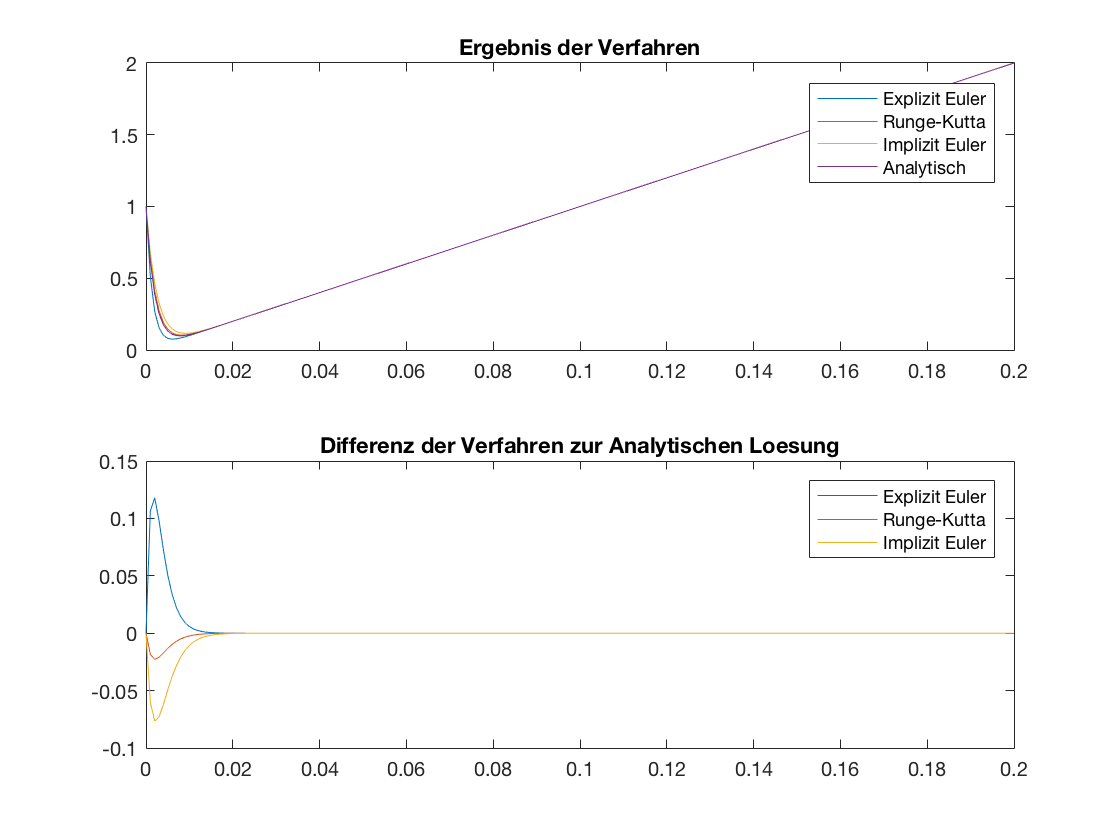
\includegraphics[width=1\linewidth]{a1_1_1}
\caption{h=0.001}
\label{fig:a1_1_1}
\end{figure}

\subsubsection{h=0.003}
Das Ergebnis zeigt, dass die Verfahren bis ca. x=0.03 unterschiedliche Ergebnisse liefern. Die Ergebnisse des Runge-Kutta-Verfahrens verlaufen bis ca. x=0.03 nahezu parallel zur analytischen Lösung. In diesem Wertebereich liefert das explizite Euler-Verfahren sehr schwankende Werte. Ab ca. x=0.03 laufen alle Kurven kongruent. Das implizite Euler Verfahren gewinnt im Gegensatz zu den anderen Verfahren durch das Steigen der Schrittweite an Genauigkeit und nähert sich in diesem Ergebnis schneller der analytischen Lösung als bei der Schrittweite von 0.001 .
\begin{figure}[htbp]
	\centering
	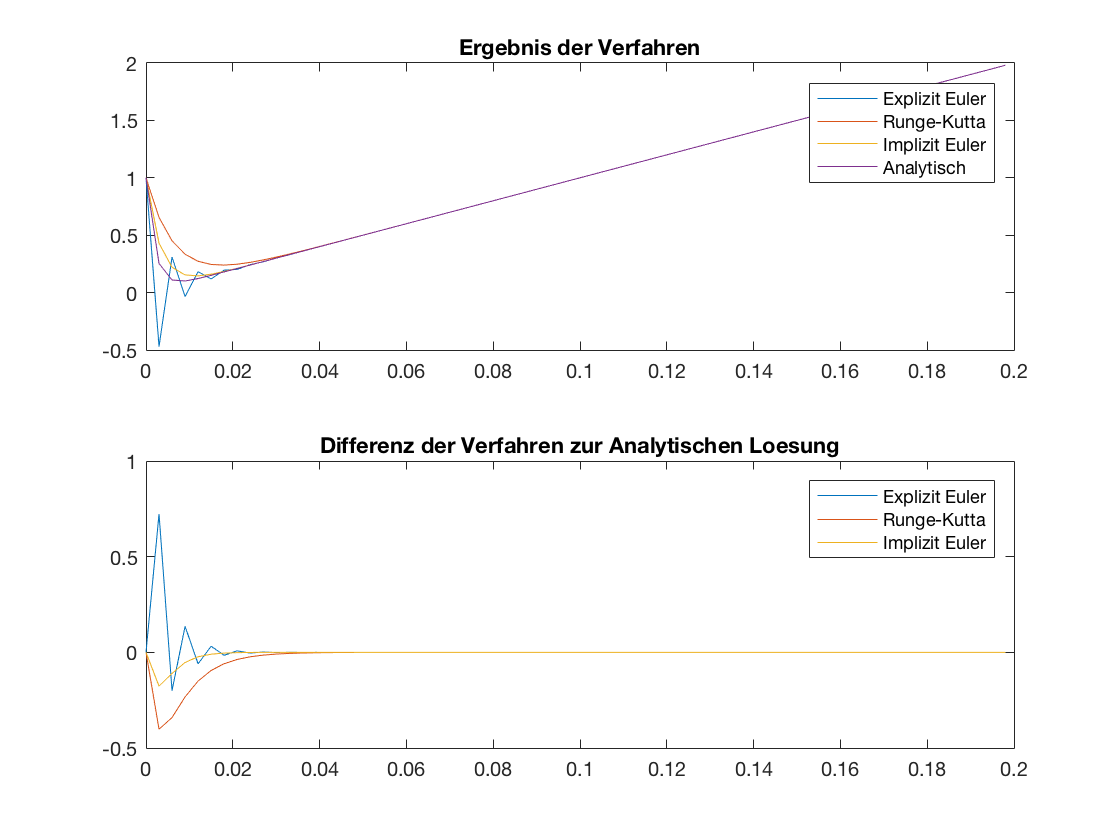
\includegraphics[width=1\linewidth]{a1_1_2}
	\caption{h=0.003}
	\label{fig:a1_1_2}
\end{figure}

\subsubsection{h=0.004}
Bis ca. x=0.01 laufen alle Kurven bis auf das des impliziten Euler Verfahrens unterschiedlich zur analytischen Lösung. Ab dort laufen die Kurven des Runge-Kutta-Verfahrens und der analytischen Lösung parallel während das implizite Euler Verfahren eine nahezu kongruente Kurve liefert. Während der ganzen Laufzeit liefert das explizite Euler-Verfahren sehr schwankende Werte, die sich mit einer Differenz von +/- 1 in der Nähe der analytischen Lösung befinden.
\begin{figure}[htbp]
	\centering
	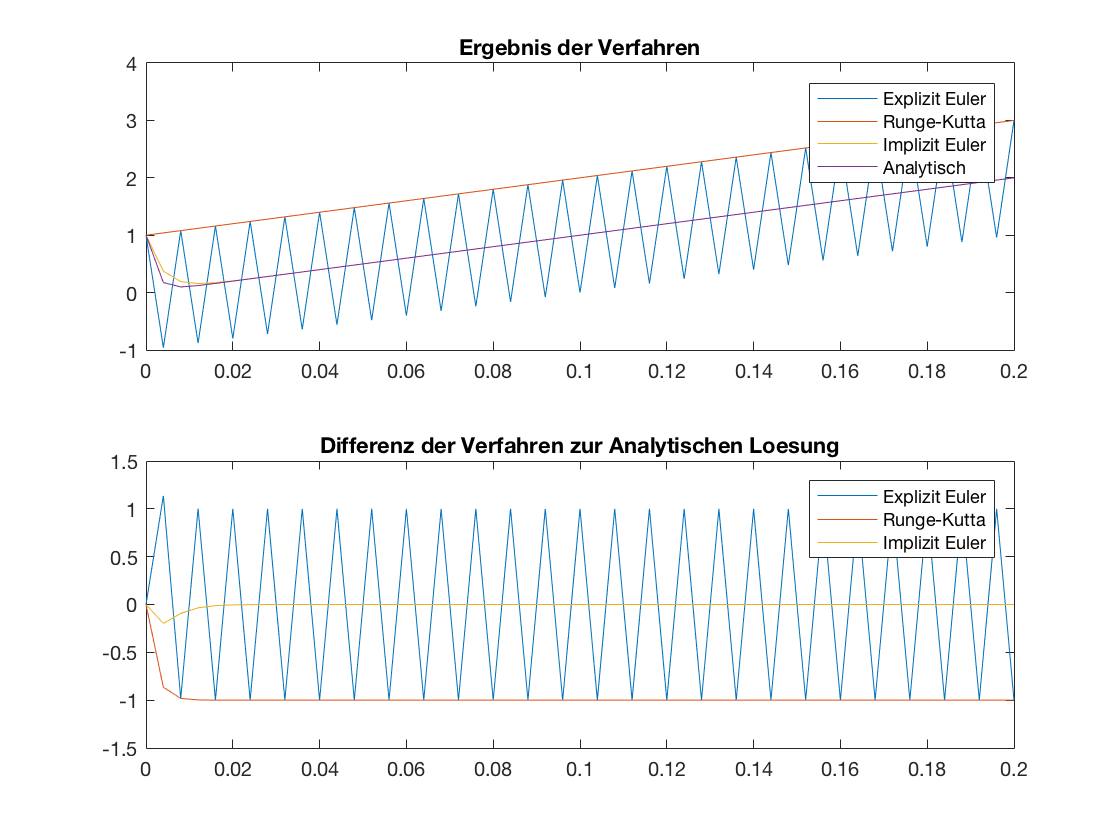
\includegraphics[width=1\linewidth]{a1_1_3}
	\caption{h=0.004}
	\label{fig:a1_1_3}
\end{figure}

\subsubsection{h=0.005}
Bis ca. x=0.15 laufen alle Kurven kongruent. Ab dort schwanken die Werte des expliziten Euler-Verfahrens mit einer Differenz von ca. +/- 0.1 um die Werte der analytischen Lösung. Die Werte des Runge-Kutta-Verfahrens hingegen werden ab ca. x=0.15 exponentiell größer und die Werte des impliziten Eulers bleiben kongruent mit der analytischen Lösung.
\begin{figure}[htbp]
	\centering
	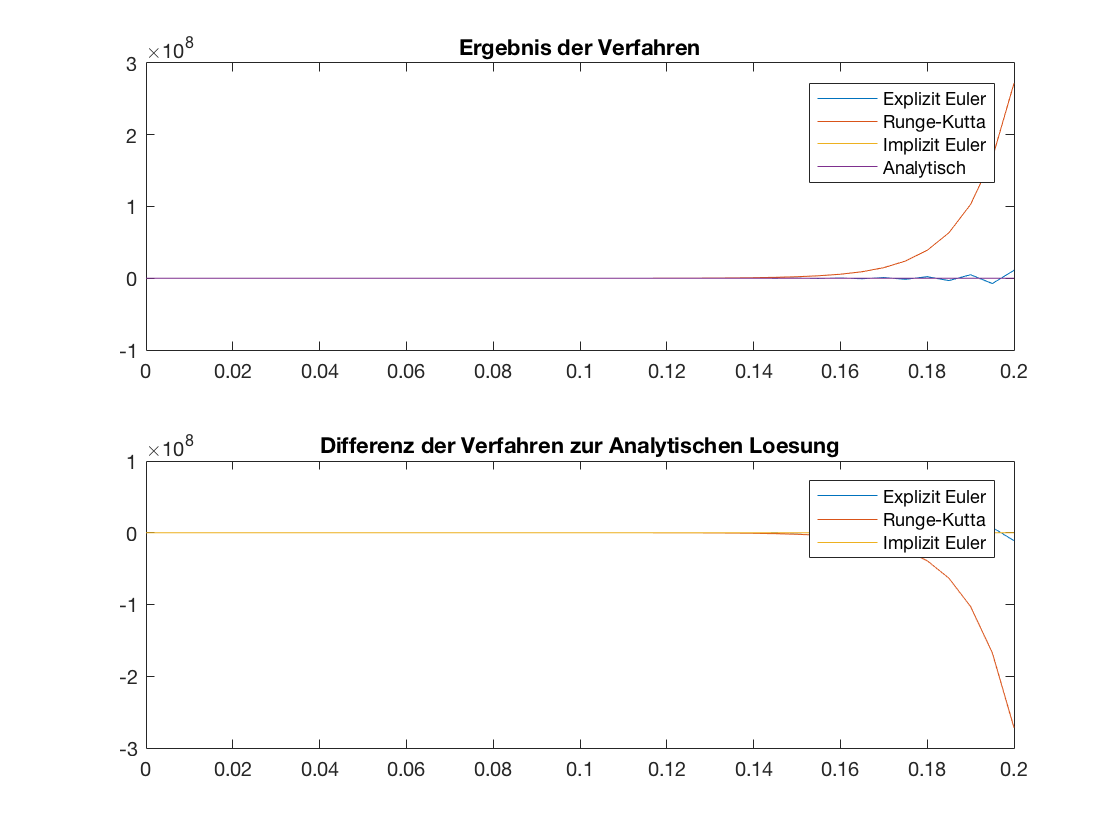
\includegraphics[width=1\linewidth]{a1_1_4}
	\caption{h=0.005}
	\label{fig:a1_1_4}
\end{figure}

\subsection{Interpretation der Ergebnisse}
Die Ergebnisse zeigen, dass die expliziten Verfahren bei einer geringen Schrittweite genauere Ergebnisse liefern. Allerdings wird dadurch die benötigte Rechenzeit erhöht. Dahingegen liefert das implizite Euler Verfahren auch bei höherer Schrittweite recht genaue Lösungen.

\section{Teilaufgabe 2 - Nicht Lineare DGL und Van der Pol}
Die folgende DGL ist gegeben: \\
$ y'' = 6 * (1 - y^{2}) * y' - y $, \\
$ y(0) = 0 $, \\
$ y'(0) = 1 $ \\

\subsection{Schaltbild}

\begin{figure}[htbp]
	\centering
	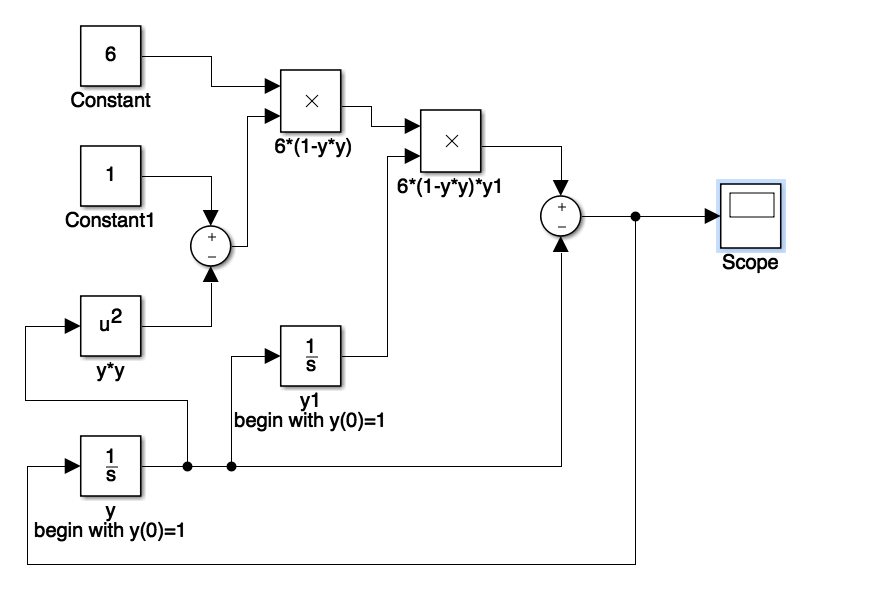
\includegraphics[width=1\linewidth]{a1_2_schaltbild}
	\caption{Simulink Schaltbild}
	\label{fig:a1_2_schaltbild}
\end{figure}

\subsection{DGLn der 1.Ordnung}
\begin{align}
\tilde{y} = y' \\
\tilde{y}' = 6 * (1 - y^{2}) * \tilde{y} - y \\
y(0)  = 0 \\
\tilde{y}(0) = 1
\end{align}

\subsection{Iterationsgleichungen}

\subsubsection{Euler-Verfahren}
\begin{align}
x_{n+1} = x_{n}+h \\
\tilde{y}_{n+1} = \tilde{y}_{n}+h*(6 * (1 - y_{n}^{2}) * \tilde{y}_{n} - y_{n}) \\
y_{n+1} = y_{n} + h * \tilde{y}_{n}
\end{align}

\subsubsection{Runge-Kutta-Verfahren 2.Ordnung}
\begin{align}
x_{n+1} = x_{n}+h \\
\tilde{k}_{1} = h * (6 * (1 - y_{n}^{2}) * \tilde{y}_{n} - y_{n}) \\
k_{1} = h * \tilde{y}_{n} \\
\tilde{k}_{2} = h * (6 * (1 - (y_{n} + \dfrac{k_{1}}{2})^{2}) * (\tilde{y}_{n} + \dfrac{\tilde{k}_{1}}{2}) - (y_{n} + \dfrac{k_{1}}{2})) \\
k_{2} = h * (\tilde{y}_{n} + \dfrac{k_{1}}{2}) \\
\tilde{y}_{n+1} = \tilde{y}_{n}+\tilde{k}_{2} \\
y_{n+1} = y_{n}+k_{2}
\end{align}

\subsection{Plot der Lösungen}
\subsubsection{h = 0.001}
\begin{figure}[H]
\centering
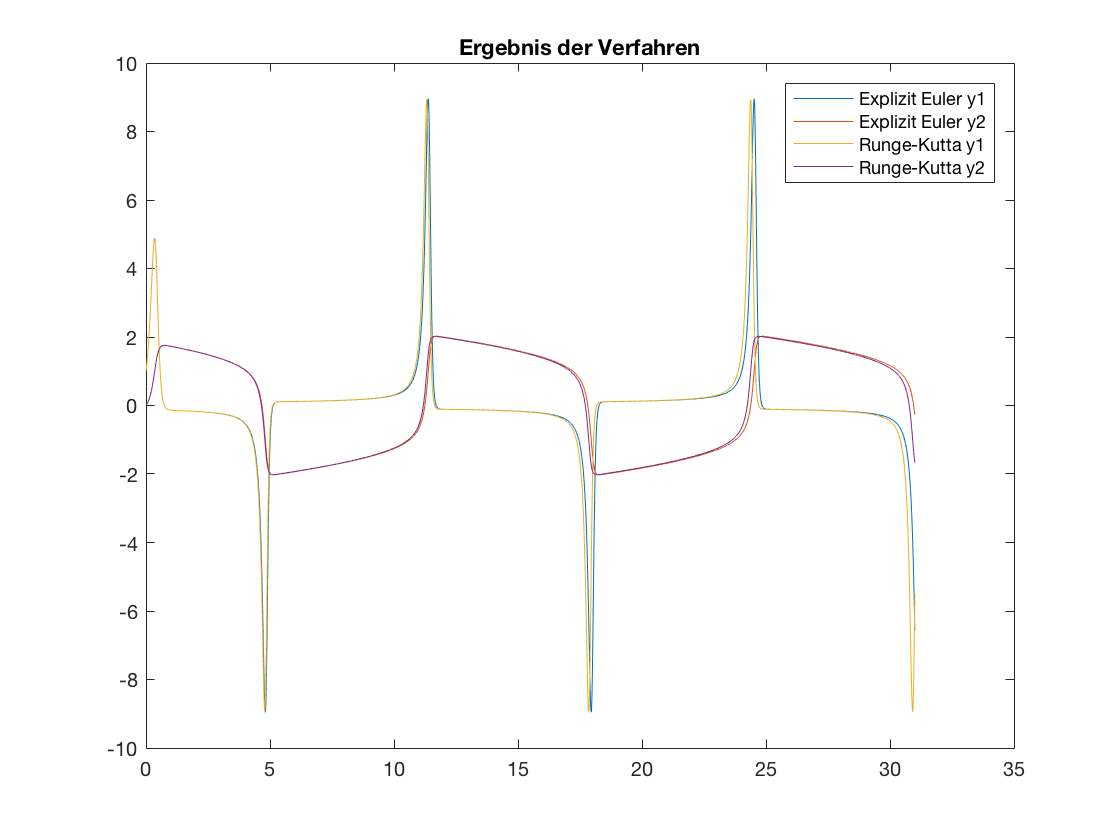
\includegraphics[width=1\linewidth]{a1_2_1}
\caption{h=0.001}
\label{fig:a1_2_1}
\end{figure}

Anhand des Ergebnisses lässt sich erkennen, dass beide Verfahren (Runge-Kutta 2.Ordnung und Expliziter Euler) bei einer Schrittweite von 0.001 kongruente Ergebnisse liefern.


\subsubsection{h = 0.02}
\begin{figure}[H]
	\centering
	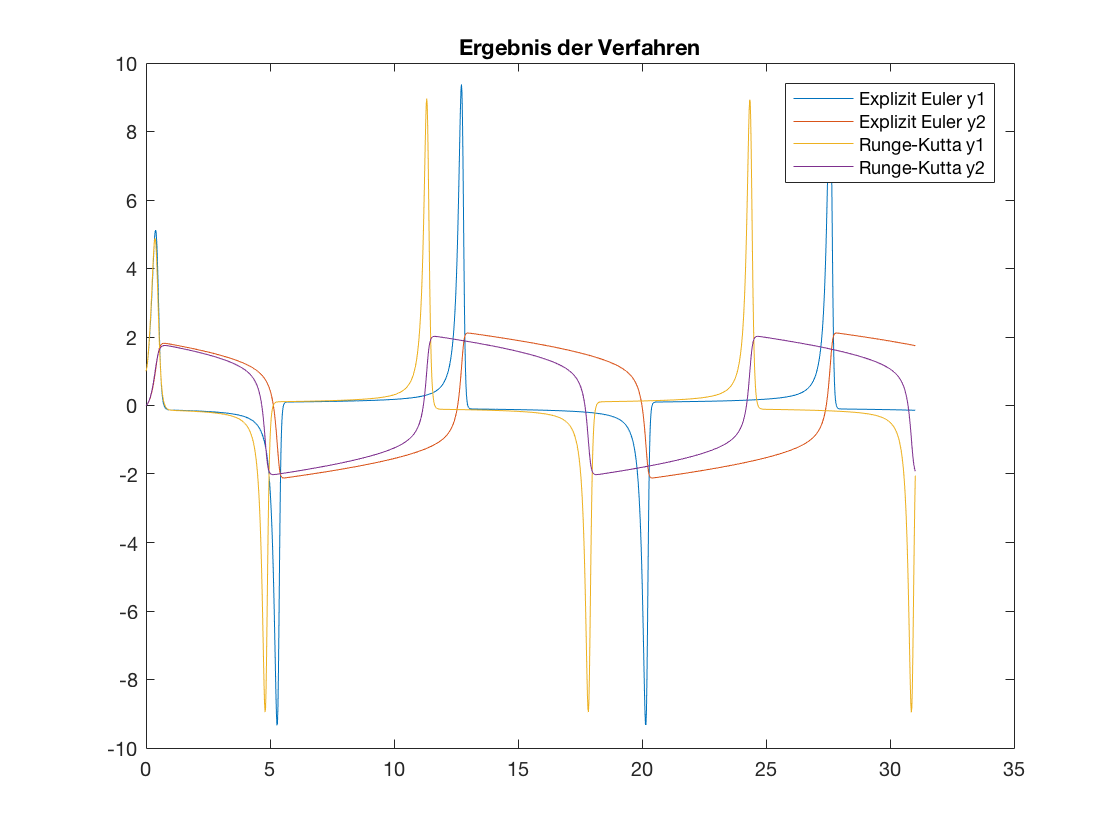
\includegraphics[width=1\linewidth]{a1_2_2}
	\caption{h=0.02}
	\label{fig:a1_2_2}
\end{figure}

In diesem Experiment mit einer Schrittweite von 0.02 verändern sich die Ergebnisse des expliziten Euler verfahrens und verschieben sich merklich gegenüber der Lösung mit einer Schrittweite von 0.001. Dahingegen verändert sich das komplexere Runge-Kutta 2. Ordnung verfahren nicht und behält das Ergebnis bei.

\section{Teilaufgabe 3 - Lorenz-Attraktor}
Es ist folgendes DGL-System gegeben: \\
$x' = -10 * (x*y)$, $x(0) = 0,01$ \\
$y' = (40 - z) * x - y$, $y(0) = 0,01$ \\
$z' = x * y - 2,67 * z$, $z(0) = 0,00$\\


\subsection{Iterationsgleichungen}
Im Folgenden die Iterationsgleichungen für das Runge-Kutta-Verfahren 2ter Ordnung bezogen auf das gegebene DGL-System.

\begin{align}
k_{1} = h * (-10 * (x_{n} * y_{n})) \\
l_{1} = h * ((40 - z) * x_{n} - y_{n}) \\
m_{1} = h * (x_{n} * y_{n} - 2,67 * z_{n}) \\
k_{2} = h*f(x_{n} + \dfrac{k_{1} }{2},y_{n} + \dfrac{l_{1} }{2},z_{n} + \dfrac{m_{1} }{2}) \\
k_{2} = h* (-10 * ((x_{n} + \dfrac{k_{1} }{2})*(y_{n} + \dfrac{l_{1} }{2})) \\
l_{2} = h*f(x_{n} + \dfrac{k_{1} }{2},y_{n} + \dfrac{l_{1} }{2},z_{n} + \dfrac{m_{1} }{2}) \\
l_{2} = h*((40 - (z_{n} + \dfrac{m_{1} }{2})) * (x_{n} + \dfrac{k_{1} }{2}) - (y_{n} + \dfrac{l_{1} }{2})) \\
m_{2} = h*f(x_{n} + \dfrac{k_{1} }{2},y_{n} + \dfrac{l_{1} }{2},z_{n} + \dfrac{m_{1} }{2}) \\
m_{2} = h*((x_{n} + \dfrac{k_{1} }{2}) * (y_{n} + \dfrac{l_{1} }{2}) - 2,67 * (z_{n} + \dfrac{m_{1} }{2})) \\
x_{n+1} = x_{n} + k2 \\
y_{n+1} = y_{n} + l2 \\
z_{n+1} = z_{n} + m2
\end{align}

\subsection{Plot der Lösung}
Gelöst durch das Runge-Kutta-Verfahren 2ter Ordnung.
\begin{figure}[H]
	\centering
	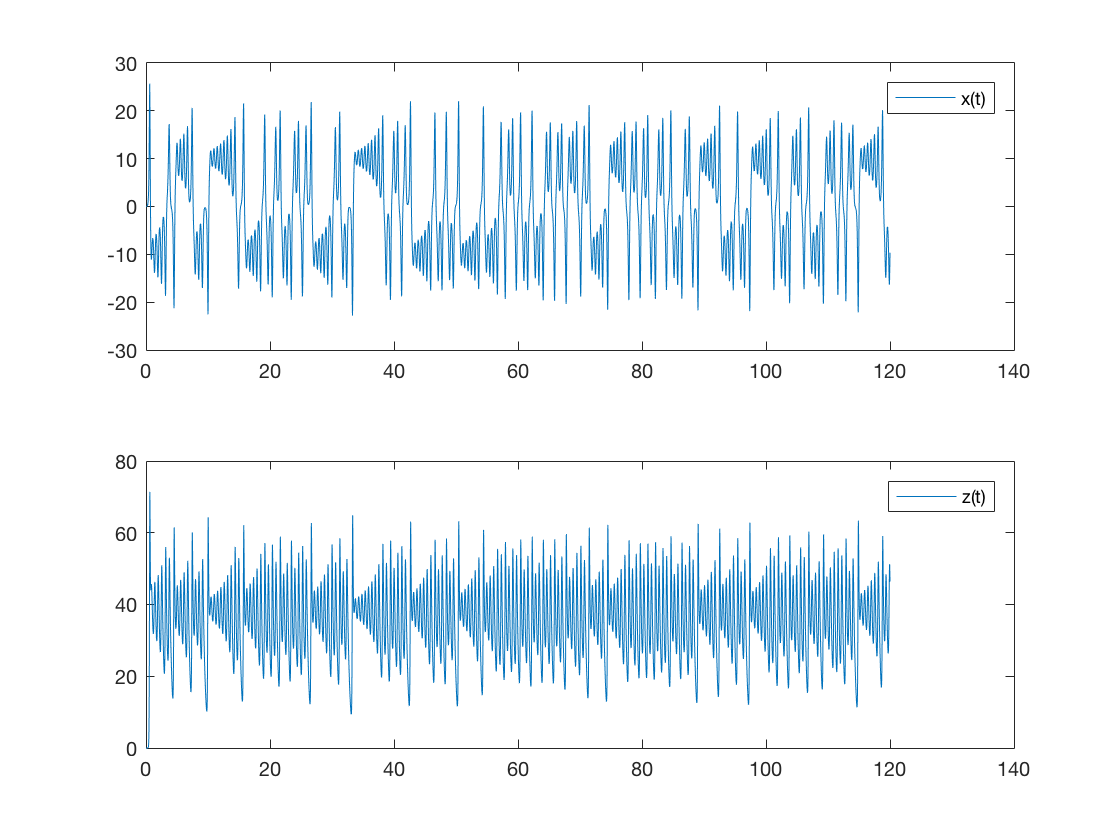
\includegraphics[width=1\linewidth]{a1_3_1}
	\caption{Vergleich von x(t) und z(t), h=0.002, $t_{end} = 120$}
	\label{fig:a1_3_1}
\end{figure}

\subsection{Schaltbild}
\begin{figure}[H]
	\centering
	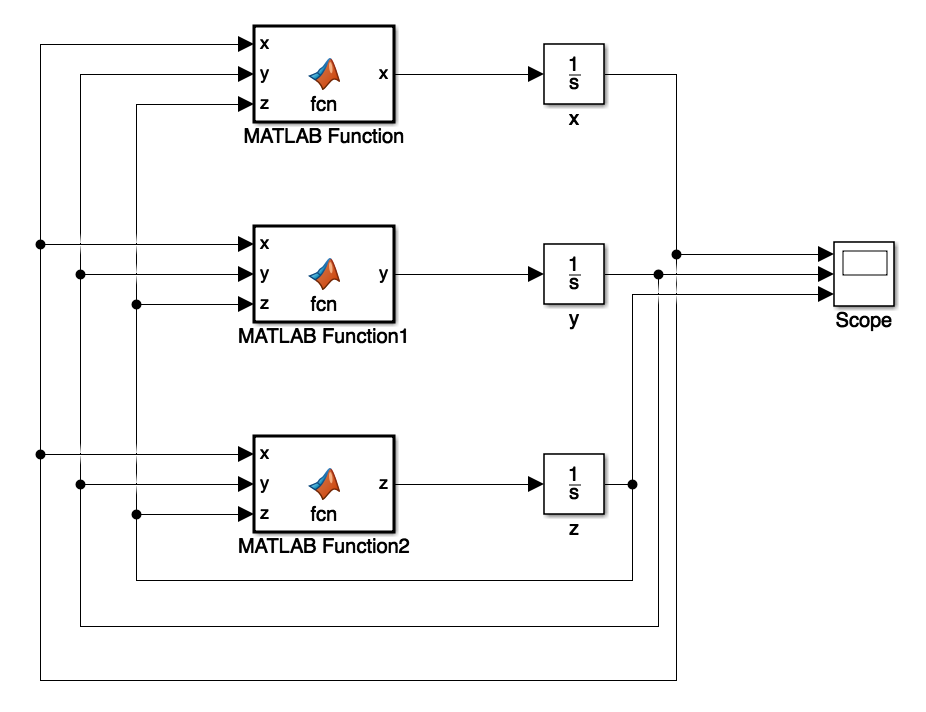
\includegraphics[width=1\linewidth]{a1_3_schaltbild}
	\caption{Simulink Schaltbild}
	\label{fig:a1_3_schaltbild}
\end{figure}

\subsection{Vergleich der Simulationen}
\begin{figure}[H]
	\centering
	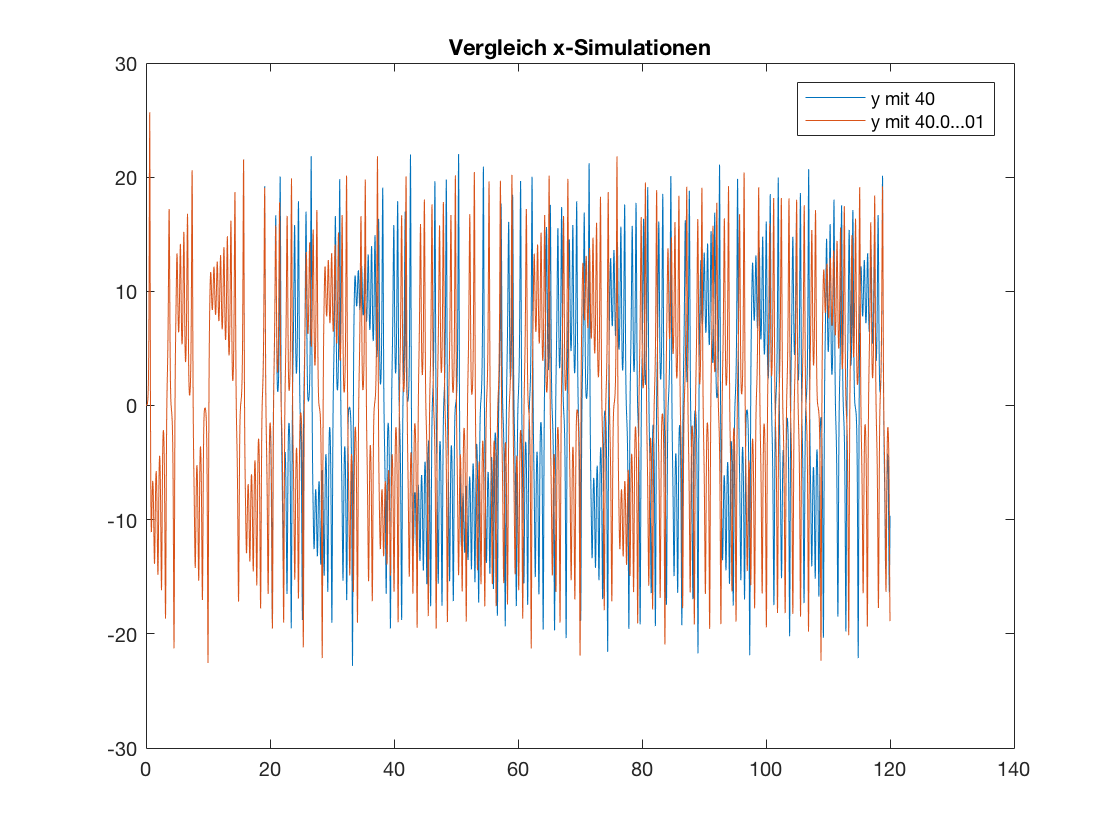
\includegraphics[width=1\linewidth]{a1_3_2}
	\caption{}
	\label{fig:a1_3_2}
\end{figure}

Durch das ausführen der zweiten Funktion y = ... mit 40.000000001 anstatt von 40 ergibt sich obenstehende Verschiebung zwischen den beiden Funktionen. Die Grafik zeigt die Lösungen des Systems mit diesem marginalen Unterschied. Aufgrund von Rundungsfehlern scheint sich die Berechnung des Systems so stark zu verändern dass sich dies in der Grafik sichtbar niederschlägt.

\end{document}
